\subsection{GWT}
The GWT front-end has several central components which facilitate interaction between the subsystems described in Design.
In the *.client package we have:
\begin{description}
\item[WebSystem] The central system which:\begin{itemize}
\item Controls how the system interacts with GAE,
\item Requests data for and loads data into the Graphical User Interface (GUI),
\item Serves as the entry point for the system, and
\item Binds the different components together.
\end{itemize}  
\item[RPC] Responsible for interacting with the Datastore via RPCs. It provides the following services:  
\begin{itemize}
\item ClassService
\item BranchProductService
\item ProductService
\item ProductCategoryService
\item LocationService
\item GeoService : Determines user location using a GWT implementation of HTML5's GeoLocation~\cite{geo} interface.
\end{itemize}
 \item[SystemData] Stores data pulled from the Datastore.
\end{description}
 In the *.client.gui.* package we have:
 \begin{description}
  \item[WebPage] Holds the various GUI components. Facilitates interaction between GUI components.
  \item[ViewTree] Provides sidebar with shortcuts to each of the major components. 
  \item[button.*] Contains custom image buttons.
    \item[loader.Loader] A loader to be displayed when the system is busy.
    \item[popup.FocusedPopupPanel] A general purpose PopupPanel which disables the background when shown.
    \item[spinedit.SpinEdit] A SpinEdit (up and down button with an IntegerBox).
    \item[table.TableView] A general purpose table display created using a FlexTable.
\end{description}
 In the *.client.util package we have:
 \begin{description}
  \item[CSSUtils] Used to inject custom css styles.
  \item[GUIUtils] Provides static access to error dialogs and the loader.
    \item[ImageUtils] Provides easy access to images.
    \item[Utils] Provides some general methods needed by some of the GUI components.
\end{description}
\subsubsection{Product Browser}
The Product Browser was implemented as follows:
\begin{description}
\item[Product Search] This was implemented as ProductSearch, a PopupPanel which allows the user to 
search for products by name, category and location. This then sends the search request
 to the Datastore via WebPage, WebSystem and RPC and directs the user to
 ProductList.
 \item[Product Viewer]This was implemented as ProductList, which presents the
 user with a tabular display of the products they searched for. It contains buttons to access ProductDetail and GraphTypePopup.
\item[Info Popup] This was implemented as ProductDetail, a popup which displays
extra information about a chosen product.
\item[Graph Chooser] This was implemented as GraphTypePopup, a PopupPanel
which allows the user choose what type of chart they which to view, in terms of
which products they wish to have displayed. This will then take the user to
the Graph Viewer.
\end{description} 
\begin{figure}[h!]
\centering
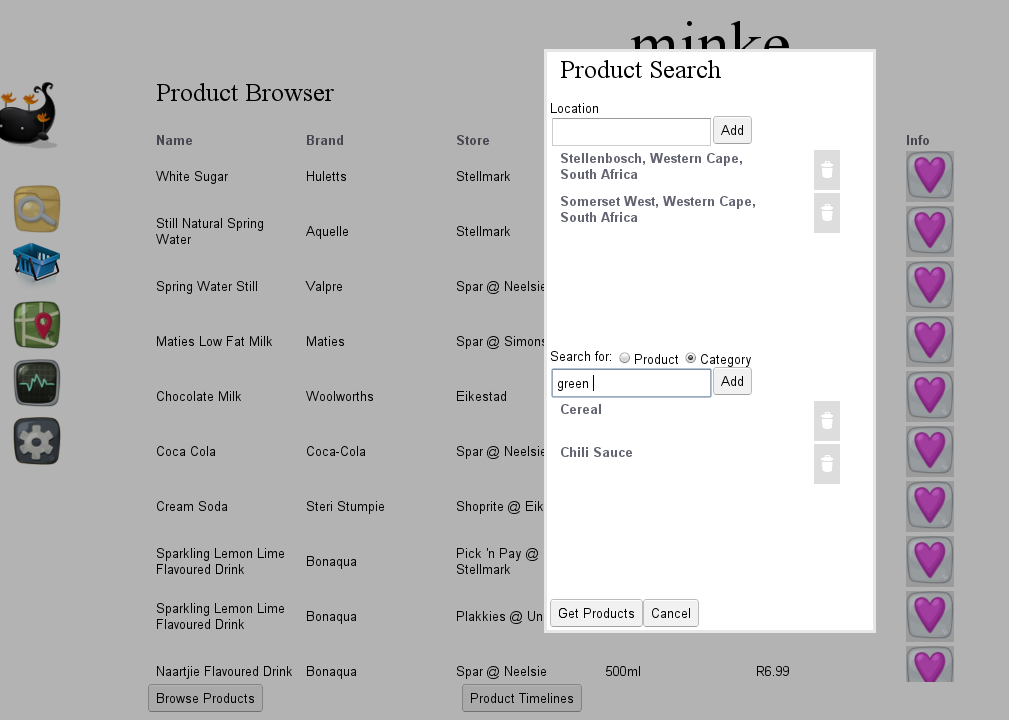
\includegraphics[width=0.8\textwidth]{gwt-search.png}
\caption{Product search interface with viewer in background.}
\end{figure}
\subsubsection{Shopping List Browser}
The Shopping List Browser was implemented using the following classes in the *.client.gui package:
\begin{description}
\item[popup.shoppinglist.ShoppingList] A popup which allows the user to add products to their shopping list via a SuggestBox~\cite{suggest}. This then sends the request for Branches which stock the products to the Datastore via WebPage, WebSystem and RPC.
\item[popup.shoppinglist.ShoppingListItem] A Composite~\cite{comp} GUI class used to represent a Product on the shopping list. Allows the user to adjust the quantity of a Product as well.
\item[table.BranchList] This presents the user with a tabular display of the Branches which stock the Products on their shopping list. This is created once the above RPC has successfully completed. It contains buttons to access ShoppingListDetail and the Directions Viewer.
\item[table.ShoppingListDetail] A table which displays the shopping list for a particular Branch. It therefore allows the user to see the price of each Product. It contains a button to access the Graph Viewer.
\item[popup.ShoppingListDetailPopup]A popup used to hold ShoppingListDetail.
\end{description}

\subsubsection{Admin Viewer}
A user is requested to enter a password before they are granted access to Admin
Viewer. The interface was implemented in the following manner:
\begin{description}
\item[Entity Chooser] This was implemented as EntityPopup, a PopupPanel with a
SuggestBox which allows the user to choose which type of entity to view. It
then requests it from the Datastore and directs the user to the DataViewer.
\item[Entity Viewer]This was implemented as DataViewer which provides the user
with a tabular view of all the entities of a particular type. It provides links
to EntityPopup and EditPopup.
\item[Entity Editor] This was implemented as EditPopup, a PopupPanel wich allows
a user to edit the various fields of a single entity or delete it completely.
After deleting or editing an entity, the DataViewer is updated with the new data
from the Datastore.
\end{description}
\begin{figure}[h!]
\centering
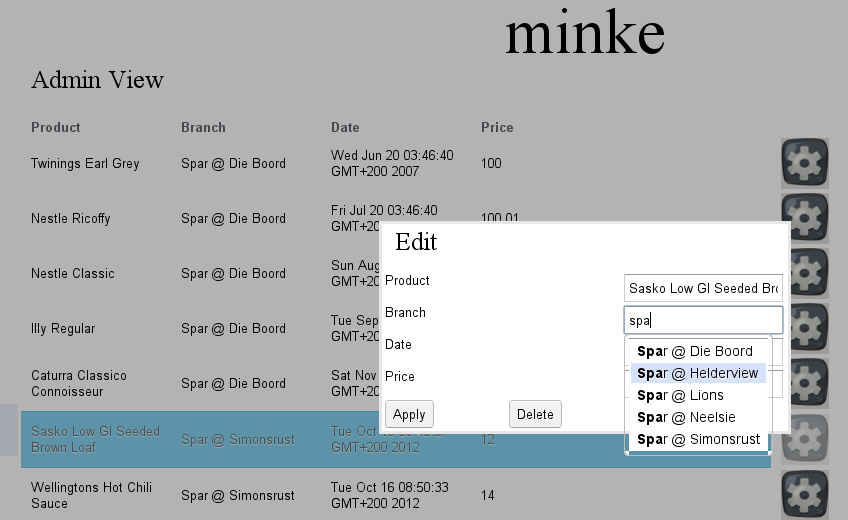
\includegraphics[width=0.8\textwidth]{gwt-admin.png}
\caption{The Entity Editor with Entity Viewer in the background.}
\end{figure}

\subsubsection{Graph Viewer}
The Graph Viewer was implemented in the following manner:
\begin{description}
\item[HistoryGraph] This was used to hold and display an instance of the
ScatterChart class as well as load the Visualization API. It also
provides a communication interface between ScatterGraph and the rest of the
system. It also allows data to be added to or removed from the current chart.
\item[ScatterGraph] A container for a ScatterChart~\cite{scatter} which loads a new chart when provided with data.
\end{description}
\begin{figure}[h!]
\centering
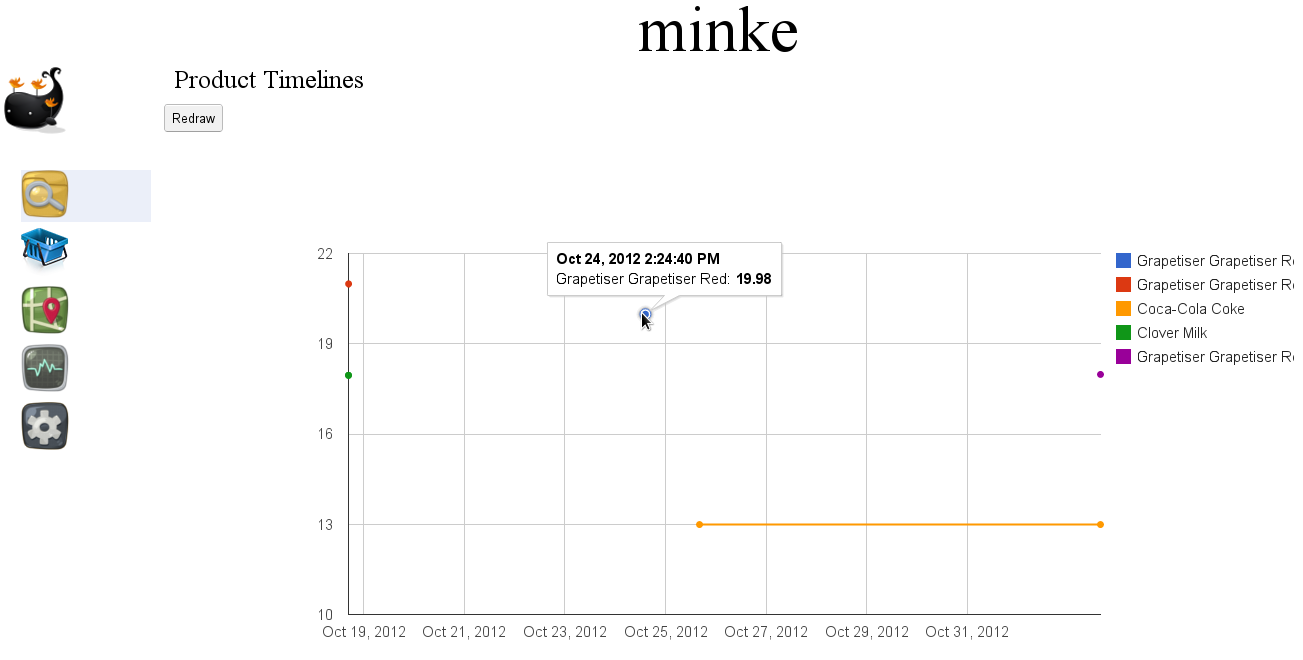
\includegraphics[width=1.0\textwidth]{gwt-graph.png}
\caption{The Graph Viewer interface.}
\end{figure}
\subsubsection{Directions Viewer}
The Directions Viewer was implemented using the following classes in the *.client.gui.map package:
\begin{description}
\item[BranchLocation] A container for the DirectionsMap class which also loads the Maps API. Also provides a communication interface between DirectionsMap and the rest of the system and allows the user to change their location.
\item[DirectionsMap] A container for a MapWidget~\cite{mwidget} and a DirectionsPanel~\cite{dpanel} which loads a new map and directions when provided with data in the form of a LatLng~\cite{latlng} map center and a String~\cite{string} containing an origin and a destination.
\end{description}

